\documentclass[a4paper,14pt]{extarticle}

% Настройка полей по ГОСТ (левое 30, правое 15, верхнее и нижнее 20)
\usepackage[left=30mm, right=15mm, top=20mm, bottom=20mm]{geometry}

% Поддержка русского языка
\usepackage[T2A]{fontenc}
\usepackage[utf8]{inputenc}
\usepackage[english,russian]{babel}

% Шрифт, похожий на Times New Roman
\usepackage{mathptmx}

% Полуторный межстрочный интервал по ГОСТ
\usepackage{setspace}
\onehalfspacing

% Абзацный отступ по ГОСТ (1.25 см)
\usepackage{indentfirst}
\setlength{\parindent}{1.25cm}

\usepackage{graphicx}

% Выравнивание текста по ширине без "рваных" краев
\tolerance=1000
\emergencystretch=2000
\begin{document}

\section{Задания 1 и 2. Разработка адаптивного интерфейса и MVC-каркаса}

В рамках первого этапа был разработан адаптивный Landing Page для образовательной платформы «EduSchool». Согласно требованиям технического задания, при верстке категорически не использовался тег \texttt{<table>} и абсолютные единицы измерения (\texttt{px}).

\subsection{Реализация адаптивной сетки (CSS Grid)}
Для отображения прайс-листа курсов был применен подход CSS Grid, обеспечивающий корректное отображение на мобильных устройствах. Для корректной работы скринридеров были добавлены семантические ARIA-роли (\texttt{role="table"}, \texttt{role="row"}).

\begin{figure}[h!]
    \centering
    % TODO: Вставить скриншот фрагмента CSS-кода с настройкой .grid-table и .table-row
    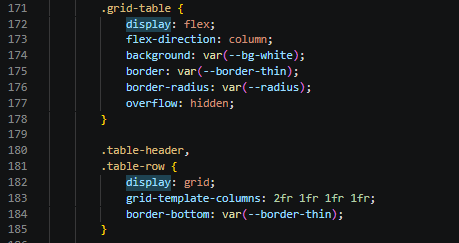
\includegraphics[width=0.8\textwidth]{скриншот_1_css_grid.png} 
    \caption{Скриншот 1: Реализация адаптивной таблицы через CSS Grid}
    \label{fig:css_grid}
\end{figure}

\subsection{Каркас Spring Boot MVC}
Был инициализирован проект на базе фреймворка Spring Boot. Реализован паттерн MVC (Model-View-Controller). Маршрутизация настроена через \texttt{HomeController} и \texttt{CourseController}, а статический HTML интегрирован в шаблонизатор Thymeleaf.

\begin{figure}[h!]
    \centering
    % TODO: Вставить скриншот дерева проекта (проводник слева), где видно папки controllers, models, templates
    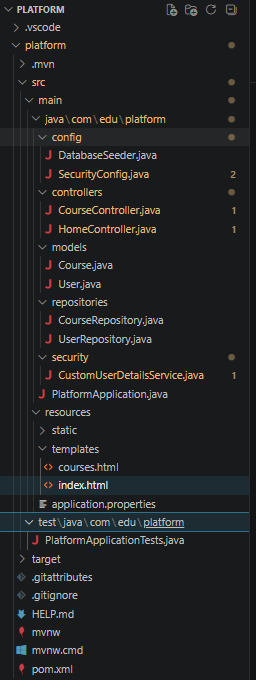
\includegraphics[width=0.5\textwidth]{скриншот_2_структура_mvc.png} 
    \caption{Скриншот 2: Структура каталогов MVC-приложения}
    \label{fig:mvc_structure}
\end{figure}

\subsection{Валидация форм (Регулярные выражения)}
На стороне клиента (Vanilla JavaScript) реализована строгая валидация полей ввода с помощью регулярных выражений.

\begin{figure}[h!]
    \centering
    % TODO: Вставить скриншот JS-кода с объектом regexPatterns
    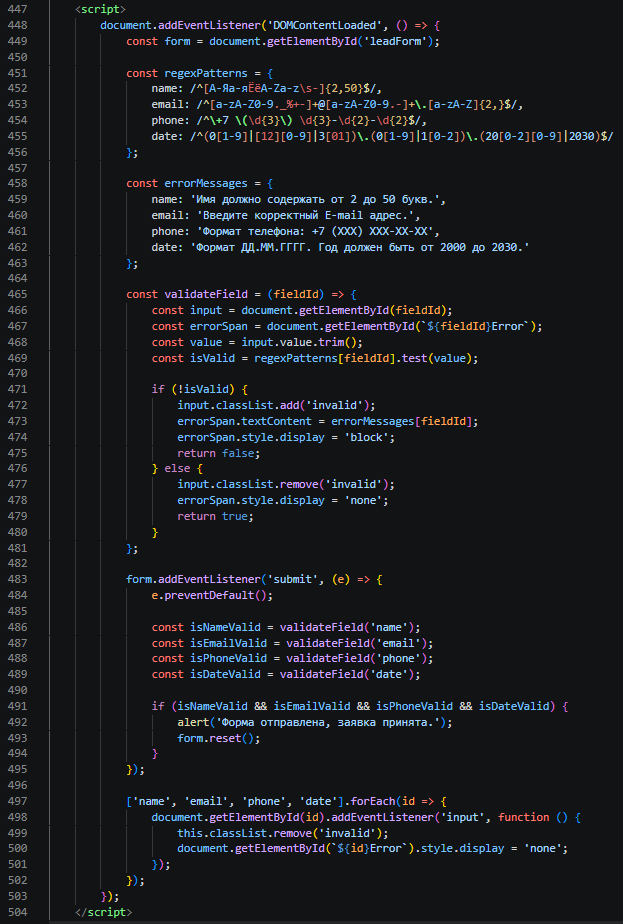
\includegraphics[width=0.9\textwidth]{скриншот_3_js_regex.png} 
    \caption{Скриншот 3: JavaScript логика клиентской валидации}
    \label{fig:js_regex}
\end{figure}

Детальный разбор разработанных регулярных выражений:

\begin{itemize}
    \item \textbf{Имя родителя:} \verb|^[А-Яа-яЁёA-Za-z\s-]{2,50}$|
    \begin{itemize}
        \item \verb|^| и \verb|$| — начало и конец строки (строгое совпадение).
        \item \verb|[...]| — разрешены русские и английские буквы, пробелы и дефис.
        \item \verb|{2,50}| — ограничение длины от 2 до 50 символов.
        \item \textit{Проходят:} Иван, Anna-Maria. \textit{Не проходят:} A (коротко), Иван123 (цифры).
    \end{itemize}

    \item \textbf{E-mail адрес:} \verb|^[a-zA-Z0-9._%+-]+@[a-zA-Z0-9.-]+\.[a-zA-Z]{2,}$|
    \begin{itemize}
        \item \verb|[a-zA-Z0-9._%+-]+| — имя ящика: буквы, цифры и спецсимволы.
        \item \verb|@| — обязательный символ "собаки".
        \item \verb|\.[a-zA-Z]{2,}| — доменная зона (точка и минимум 2 буквы).
        \item \textit{Проходят:} test@mail.ru. \textit{Не проходят:} test.ru (нет @).
    \end{itemize}

    \item \textbf{Номер телефона:} \verb|^\+7 \(\d{3}\) \d{3}-\d{2}-\d{2}$|
    \begin{itemize}
        \item \verb|\+7 \(| — экранированные символы кода страны и открывающей скобки.
        \item \verb|\d{3}| — ровно 3 цифры (код оператора).
        \item \verb|\d{3}-\d{2}-\d{2}| — блоки цифр, разделенные дефисами.
        \item \textit{Проходят:} +7 (999) 123-45-67. \textit{Не проходят:} 89991234567 (неверный формат).
    \end{itemize}

    \item \textbf{Дата начала обучения:} \verb|^(0[1-9]|[12][0-9]|3[01])\.(0[1-9]|1[0-2])\.(20[0-2][0-9]|2030)$|
    \begin{itemize}
    
        \item \verb|(0[1-9]|[12][0-9]|3[01])| — валидация дня (от 01 до 31).
        \item \verb|(0[1-9]|1[0-2])| — валидация месяца (от 01 до 12).
        \item \verb|(20[0-2][0-9]|2030)| — ограничение года строго от 2000 до 2030.
        \item \textit{Проходят:} 27.03.2026. \textit{Не проходят:} 32.01.2024 (неверный день).
    \end{itemize}
\end{itemize}

\section{Задание 3. Интеграция базы данных, ORM и маршрутизация}

В данном разделе реализовано подключение приложения к СУБД PostgreSQL, внедрение ORM-системы на базе Spring Data JPA и настройка динамического рендеринга данных на стороне сервера.

\subsection{Настройка подключения и подход Code First}
Для взаимодействия с базой данных использовался паттерн проектирования Code First. В конфигурационном файле \texttt{application.properties} заданы параметры подключения к PostgreSQL и активировано свойство \texttt{spring.jpa.hibernate.ddl-auto=update}. Это позволило фреймворку автоматически генерировать и обновлять структуру реляционных таблиц на основе Java-классов без ручного написания DDL-скриптов.

\begin{figure}[h!]
    \centering
    % TODO: Скриншот файла application.properties
    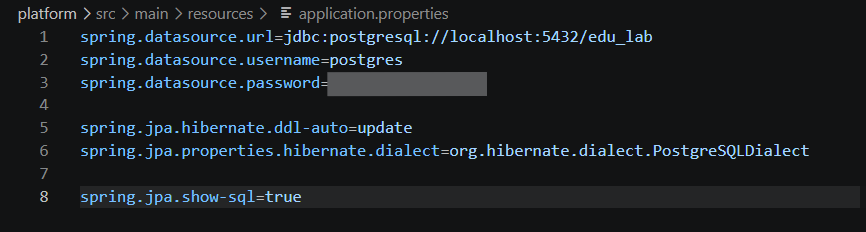
\includegraphics[width=0.9\textwidth]{скриншот_4_app_properties.png} 
    \caption{Скриншот 4: Конфигурация подключения и настройка Hibernate}
    \label{fig:app_properties}
\end{figure}

\subsection{Разработка моделей и репозиториев (JPA)}
Была создана доменная сущность \texttt{Course}, размеченная аннотациями \texttt{@Entity} и \texttt{@Table}. Для абстрагирования логики доступа к данным (Data Access Object) создан интерфейс \texttt{CourseRepository}, наследующий \texttt{JpaRepository}. Это обеспечило приложение готовыми методами CRUD (Create, Read, Update, Delete) без необходимости написания SQL-запросов вручную.

\begin{figure}[h!]
    \centering
    % TODO: Скриншот класса Course.java с аннотациями
    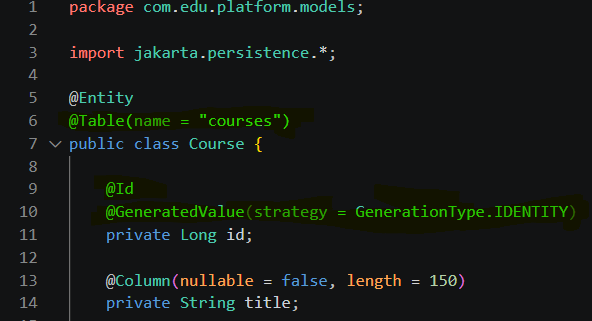
\includegraphics[width=0.8\textwidth]{скриншот_5_course_entity.png} 
    \caption{Скриншот 5: Реализация сущности Course с аннотациями JPA}
    \label{fig:course_entity}
\end{figure}

\subsection{Маршрутизация (Routing) и контроллеры}
Для выполнения требований по добавлению новых роутов маршрутизация приложения была расширена. Настроен контроллер \texttt{CourseController}, обрабатывающий GET-запросы по пути \texttt{/courses}. Контроллер внедряет в себя репозиторий, извлекает список курсов из базы данных и передает его в представление через объект \texttt{Model}.

\subsection{Динамический рендеринг представлений (Thymeleaf)}
Статическая верстка прайс-листа была заменена на динамическую генерацию. С помощью шаблонизатора Thymeleaf и атрибута \texttt{th:each} реализован цикл, который проходит по переданной коллекции курсов и автоматически формирует строки CSS Grid таблицы, подставляя в них данные из БД.

\begin{figure}[h!]
    \centering
    % TODO: Скриншот HTML-кода с циклом th:each
    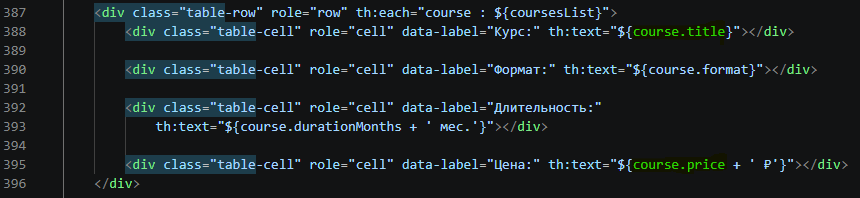
\includegraphics[width=0.9\textwidth]{скриншот_6_thymeleaf_each.png} 
    \caption{Скриншот 6: Динамическая генерация таблицы прайс-листа}
    \label{fig:thymeleaf_each}
\end{figure}

\begin{figure}[h!]
    \centering
    % TODO: Скриншот окна браузера с рабочим сайтом (страница /courses или прайс-лист)
    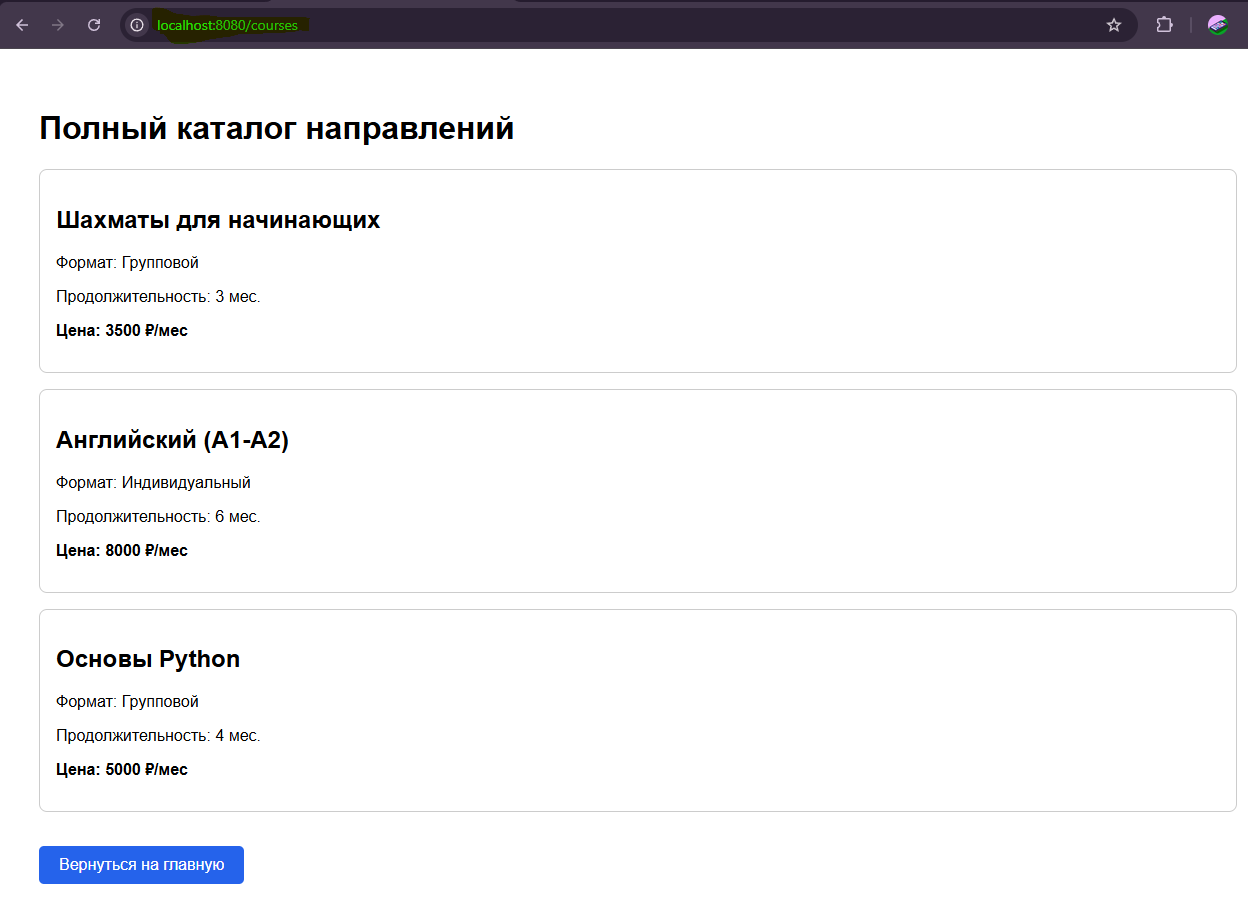
\includegraphics[width=1\textwidth]{скриншот_7_browser_courses.png} 
    \caption{Скриншот 7: Результат динамического вывода данных из БД на страницу}
    \label{fig:browser_courses}
\end{figure}

\section{Задания 4 и 5. Безопасность, роли и управление состоянием}

На завершающем этапе разработки была реализована подсистема аутентификации и авторизации пользователей, а также механизм сохранения состояния сеанса, что удовлетворяет требованиям к ограничению доступа и работе с сессиями.

\subsection{Интеграция Spring Security и аутентификация}
Для обеспечения безопасности приложения был подключен модуль \texttt{spring-boot-starter-security}. В базе данных создана таблица \texttt{users} (модель \texttt{User}), хранящая логины, зашифрованные пароли и роли пользователей (например, \texttt{ROLE\_ADMIN}, \texttt{ROLE\_USER}). 

Шифрование паролей осуществляется с использованием стойкого криптографического алгоритма \texttt{BCryptPasswordEncoder}. Для валидации учетных данных был реализован сервис \texttt{CustomUserDetailsService}, переопределяющий метод \texttt{loadUserByUsername}, который осуществляет поиск пользователя в базе данных через \texttt{UserRepository}.

\begin{figure}[h!]
    \centering
    % TODO: Скриншот файла SecurityConfig.java (настройка ролей)
    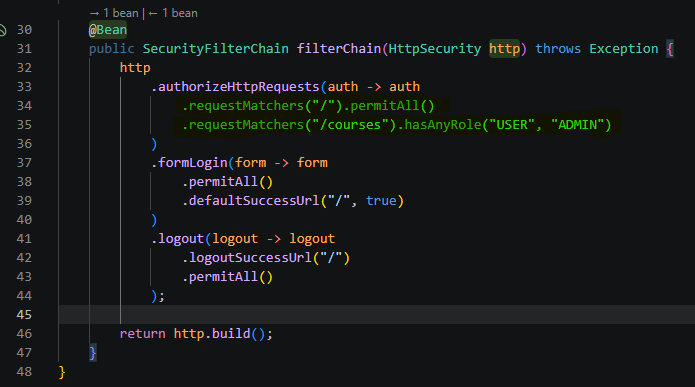
\includegraphics[width=0.9\textwidth]{скриншот_8_security_config.png} 
    \caption{Скриншот 8: Конфигурация цепочки фильтров безопасности (SecurityFilterChain)}
    \label{fig:security_config}
\end{figure}

\subsection{Авторизация и ограничение доступа по ролям}
В конфигурационном классе \texttt{SecurityConfig} были настроены правила авторизации (URL Authorization). 
Применено строгое разделение прав:
\begin{itemize}
    \item Маршрут \texttt{/} (Landing Page) доступен всем посетителям сайта (\texttt{permitAll()}).
    \item Маршрут \texttt{/courses} (Каталог курсов) защищен и доступен только аутентифицированным пользователям с правами \texttt{USER} или \texttt{ADMIN} (\texttt{hasAnyRole()}).
\end{itemize}
Попытка доступа неавторизованного пользователя к защищенным ресурсам автоматически перенаправляет его на форму логина.

\subsection{Работа с состоянием приложения (Session \& Cookies)}
Для реализации сохранения состояния (Задание 5) использованы механизмы HTTP-сессий и Cookie. При успешной аутентификации Spring Security создает серверную сессию (\texttt{HttpSession}) и отправляет браузеру идентификатор \texttt{JSESSIONID} в виде Cookie.

Для демонстрации работы состояния на клиентской части был интегрирован диалект \texttt{thymeleaf-extras-springsecurity6}.

\begin{figure}[h!]
    \centering
    % TODO: Скриншот HTML-кода шапки с sec:authorize
    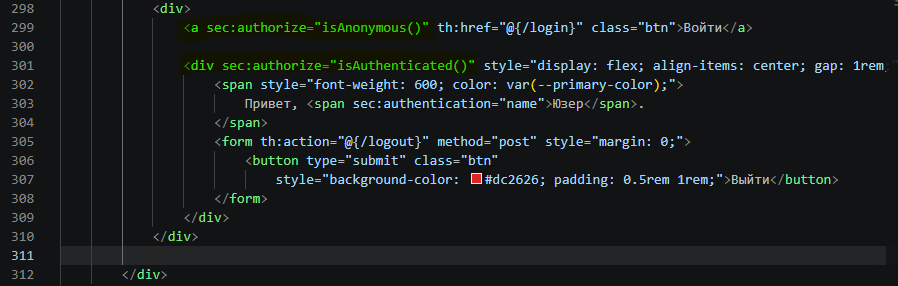
\includegraphics[width=0.8\textwidth]{скриншот_9_thymeleaf_security.png} 
    \caption{Скриншот 9: Динамическое изменение интерфейса на основе состояния сессии}
    \label{fig:thymeleaf_security}
\end{figure}

Навигационное меню динамически реагирует на статус сессии:
\begin{itemize}
    \item При отсутствии сессии (\texttt{isAnonymous()}) отображается кнопка «Войти».
    \item При наличии валидной сессии (\texttt{isAuthenticated()}) отображается имя текущего пользователя (\texttt{sec:authentication="name"}) и кнопка «Выйти». 
\end{itemize}
Выход из системы (\texttt{/logout}) реализован через метод \texttt{POST} (для защиты от CSRF-атак). При выходе сессия инвалидируется, а Cookie затирается, возвращая приложение в исходное состояние.

\begin{figure}[h!]
    \centering
    % TODO: Скриншот браузера с авторизованным юзером (видна шапка с "Привет, admin")
    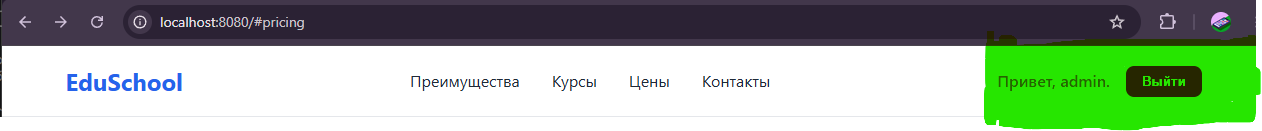
\includegraphics[width=1\textwidth]{скриншот_10_logged_in.png} 
    \caption{Скриншот 10: Интерфейс приложения после успешной аутентификации пользователя}
    \label{fig:logged_in}
\end{figure}
\end{document}
